\documentclass[twocolumn]{article}
\usepackage{graphicx} % Required for inserting images
\usepackage{listings}
\title{Utilizing a wet/dry sensor as a salinity sensor}
\author{Jordan Reichhardt\\California Polytechnic State University\\jreichha@calpoly.edu}
\date{August 2023}

\begin{document}

\maketitle


\section{abstract}
The salinity of the oceans provides telling metrics about ocean health, including indications of current and levels of ocean warming. Unfortunately, salinity is difficult to measure within the surf zone because buoys are often unreliable. For this reason, developing a salinity sensor to integrate with Smartfin would allow scientists to better analyze salinity levels along all coasts. Here,an experiment for testing a salinity sensor by utilizing the circuitry of our wet/dry sensor is detailed. A solution for the shortcomings of the sensor is also proposed.


\maketitle

\section{Introduction}
We have developed an experiment to test the wet/dry sensor's circuitry and determine if we can utilize this circuitry to measure salinity. In this experiment, we test water with salinity ranging from 33,000 parts per million (ppm) to 37,000 ppm, which is the typical salinity range for ocean water. This is tested in increments of 250 ppm to determine if we can read a small enough change in salinity. If this level of precision is met, we will continue the experiment again with smaller increments.

\section{Materials}
\begin{itemize}
    \item  Picoscope or oscilloscope and function generator
    \item Power source
    \item 3 BNC to grabber probes (for the oscilloscope and function generator)
    \item 2 banana to grabbers (for power)
    \item Smartfin PCB for E Series board
    \item Jumper wires
    \item 2 gallons of distilled water
    \item 4 cups of salt
\end{itemize}

\section {Salinity ratios}
Table \ref{tab:salinity_measurements} shows the ratio of salt to water needed to create jars with a range of salinity from 33,000 ppm to 37,000 ppm in increments of 250 ppm. This range of salinities allows for adequate testing of the precision of the wet/dry sensor as a salinity sensor.


\section{Picoscope settings}
\begin{itemize}
    \item Function generator on square wave at 1 kHz
    \item Both probes at 5 V (allows us to read 3.3 V)
\end{itemize}

\begin{table}[ht]
    \caption{Salinity measurements}
    \centering
    \begin{tabular}{lll}
        \hline
        Salinity (ppm) & Water (mL) & Salt (g) \\ \hline
        33,000         & 400               & 16.0             \\
        33,250         & 400               & 16.1             \\
        33,500         & 400               & 16.2             \\
        33,750         & 400               & 16.4             \\
        34,000         & 400               & 16.5             \\
        34,250         & 400               & 16.6             \\
        34,500         & 400               & 16.7             \\
        34,750         & 400               & 16.9             \\
        35,000         & 400               & 17.0             \\
        35,250         & 400               & 17.1             \\
        35,500         & 400               & 17.2             \\
        35,750         & 400               & 17.4             \\
        36,000         & 400               & 17.5             \\
        36,250         & 400               & 17.6             \\
        36,500         & 400               & 17.7             \\
        36,750         & 400               & 17.9             \\
        37,000         & 400               & 18.0             \\ \hline
    \end{tabular}
    \label{tab:salinity_measurements}
\end{table}

\section{Procedure}
\subsection{Picoscope Setup}
\begin{itemize}
    \item Connect the Picoscope to a laptop and be sure to have Picoscope 7 T\&M (version may vary)\footnote{https://www.picotech.com/downloads} installed on your laptop beforehand.
    \item Connect the function generator line of the Picoscope to the \lstinline{WATER EN} wire of the PCB
          \begin{itemize}
              \item The first probe goes to the \lstinline{WATER EN} is in order to verify the function generator waveform is inputting correctly to \lstinline{WATER EN}
              \item The second probe goes to the \lstinline{COMP MINUS} (before doing this you may want to check that the \lstinline{WATER} wire, the output of the comparator opamp is at 3.3V)
          \end{itemize}
    \item Attach a power source to the \lstinline{3V3} line and ground the board. (there should be a common ground between all scope probes and the ground on the board).
\end{itemize}

\subsection{Oscilloscope/Function Generator Setup}
\begin{itemize}
    \item Attach a function generator to \lstinline{WATER EN}.
    \item Attach a probe on the oscilloscope to \lstinline{WATER EN} and verify the waveform from the function generator
    \item Attach the second oscilloscope probe to the \lstinline{COMP MINUS} (before doing this you may want to check that the \lstinline{WATER} wire, the output of the comparator opamp is at 3.3V)
\end{itemize}

\subsection{Measurements}
\begin{itemize}
    \item Begin the measurements (from Table \ref{tab:salinity_measurements}) with large increments and get smaller. In other words, start measuring if there is a noticeable difference between the 33,000 ppm water and the 37,000 ppm water and then continue to move inwards on the chart.
    \item Record the voltage differences for each of the varying salinity. We will then use this voltage to calculate the salinity.
\end{itemize}

\begin{figure}
    \centering
    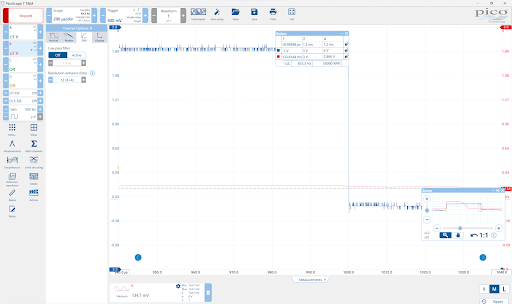
\includegraphics[width=0.4\textwidth]{34,000ppmsalinity.png}
    \caption{Voltage output from \lstinline{COMP MINUS} at 34,000 ppm salinity}
    \label{fig:salinity_34000}
\end{figure}

\begin{figure}
    \centering
    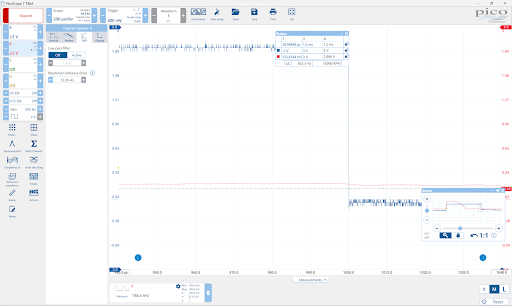
\includegraphics[width=0.4\textwidth]{36,000ppmsalinity.png}
    \caption{Voltage output from \lstinline{COMP MINUS} at 36,000 ppm salinity}
    \label{fig:salinity_36000}
\end{figure}

\subsection{Results}
We began our tests with 34,000 and 36,000 ppm of salt. The oscilloscope readings from these salinity levels are shown in Figure \ref{fig:salinity_34000} and \ref{fig:salinity_36000}. The voltage difference between the 34,000 ppm and 36,000 ppm was not great enough to indicate that the wet/dry circuitry is currently in a sufficient state to function as a salinity sensor. One possible way to alter the wet/dry circuit in order to get a large enough voltage out of the \lstinline{COMP MINUS} to determine a change in salinity is to decrease the resistor value on the positive rail of the opamp. This change would increase the voltage to the water detect pad, creating larger increments in voltage change between solutions of different salinity. The goal of this increase in voltage is to create a clearer voltage increment, which would better show changing salinity.



\end{document}
